\vspace{3cm}

\begin{center}
    \textbf{Susana Flecha$^{1,2}$, Àlex Giménez-Romero$^{3}$, Joaquín
        Tintoré$^{2,4}$, Fiz F. Pérez$^{5}$, Eva Alou-Font$^{4}$, Manuel A.
        Matías$^{3}$, Iris E. Hendriks$^{2}$}
\end{center}

\vspace{1cm}

\begin{enumerate}
    \small
    \item Instituto de Ciencias Marinas de Andalucía (ICMAN-CSIC), Polígono Río
          San Pedro s/n, 11519 Cádiz, Puerto Real, Spain.
    \item Instituto Mediterráneo de Estudios Avanzados, IMEDEA (CSIC-UIB),
          E-07190 Esporles, Mallorca, Spain.
    \item Instituto de Física Interdisciplinar y Sistemas Complejos, IFISC
          (CSIC-UIB), Palma de Mallorca 07122, Spain.
    \item Balearic Islands Coastal Observing and Forecasting System (SOCIB),
          Parc Bit, Naorte, Bloc A 2op. pta. 3, 07121 Palma, Spain
    \item Instituto de Investigaciones Marinas (IIM-CSIC), Eduardo Cabello 6,
          36208 Vigo, Spain.
\end{enumerate}

\vspace{1cm}

\textbf{Published as}

\vspace{0.5cm}

\fullcite{Flecha2022}

\newpage
\section{Introduction}

Atmospheric carbon dioxide (CO\textsubscript{2}) emissions are
exponentially increasing since the industrial revolution, principally due to
fossil fuel use, industry and land-use change. Around a 46\% of this
CO\textsubscript{2} remains in the atmosphere while the rest is captured by
natural compartments: the terrestrial biosphere and the
ocean\cite{Friedlingstein2021}.  At present, the oceans have absorbed around an
estimated 26\% of the total anthropogenic CO\textsubscript{2} released from
2011 to 2020 \cite{Friedlingstein2021}. Once CO\textsubscript{2} dissolves in
seawater, a sequence of chemical reactions occurs that derives in an increase
of [H\textsuperscript{+}] ions, which results in a decrease in seawater pH.
This process, a consequence of increasing atmospheric CO\textsubscript{2}, is
termed Ocean Acidification (OA)\cite{caldeira2003anthropogenic}. In addition to
the pH decrease, [H\textsuperscript{+}] ions react with carbonate ions
    [CO\textsubscript{3}\textsuperscript{2-}] to form
    [HCO\textsubscript{3}\textsuperscript{-}], leading to a reduction of the
    [CO\textsubscript{3}\textsuperscript{2-}] ion levels \cite{doney2009ocean}.
Low
carbonate levels affect the saturation state of calcium carbonate minerals,
increasing difficulties in shell-forming for calcifying marine organisms (e.g.,
plankton, mollusks, echinoderms and corals). Consequences of OA are an
important threat to marine ecosystems visible in higher levels of the trophic
chain, with complex and wide-ranging impacts on the physiology of different
species and therefore on their
metabolism\cite{kroeker2013impacts,nilsson2012near}. These metabolic effects
will have numerous consequences at an organism scale, in particular, they can
cause a decrease in growth, locomotion, reproductive capacity and homeostasis
if they are not capable to control the conditions for
calcification\cite{hendriks2015biological}. Negative effects of this magnitude
could cause an unexpected cascade effect impacting on the structure and
functions of ecosystems and trophic networks\cite{zunino2021impact} and cannot
be easily generalized.\\
Also, ocean CO\textsubscript{2} uptake and derived OA are not homogeneous
at the global scale, with some areas more affected. For instance, the
Mediterranean Basin is an area where effects are stronger compared to the
global ocean\cite{Giorgi2006}. The Mediterranean Sea, constituting only a
0.82\% of the surface and 0.32\% of the volume of the global ocean, is
cataloged as one of the most complex marine ecosystems, defined as a “miniature
ocean”\cite{bethoux1999mediterranean}, inhabited by an extensive and diverse
biota that represents between 4 and 18 \% of the world's total marine species
\cite{Bianchi2000} and serves as a model\cite{bethoux1999mediterranean} to
anticipate the responses of the global ocean to different types of pressures.
It has been also defined as a climate change ``hot spot'' \cite{Giorgi2006},
whit OA and its derived consequences characterized as one of the climatic
threats with the greatest potential impact, followed by the temperature and UV
radiation increase \cite{micheli2013}. The temperature rise in this
semi-enclosed sea is expected to be two to four-fold times higher than that in
the global ocean \cite{vargas2008w, vargas2010}. In addition, the sixth
assessment report (AR6) of the IPPC7, places a high level of confidence on the
increase in frequency of heatwaves and ongoing ocean
acidification\cite{Masson-Delmotte2021}. Recent studies have confirmed that
there is a trend of around 0.34 °C warming per decade in the Mediterranean
Outflow Water (MOW) through the Strait of Gibraltar towards the Atlantic Ocean
\cite{Garcia-Lafuente2021}, associated with decreasing values of pH.
Furthermore, in the Mediterranean Sea, due to its biogeochemical and
hydrodynamic characteristics, such as the high alkalinity of its waters and the
active thermohaline circulation \cite{Alvarez2014}, there is a larger
absorption of atmospheric CO\textsubscript{2} and an intense transport of this
CO\textsubscript{2} from the oceanic surface to deep
areas\cite{Hassoun2015,Palmieri2015}, already observed in the MOW
\cite{Flecha2015,Flecha2019}, with estimated OA trends of -0.0044 pH units per
year in the Strait of Gibraltar \cite{Flecha2015} and ranging from -0.0017 to
-0.003 in the Mediterranean Basin\cite{Kapsenberg2017,yao2016}.\\
The Mediterranean Sea has an extensive coastline, which extends for
$\SI{46000}{km}$ and is shared by 21 countries \cite{EEA1999}. Coastal zones,
as transitional areas, are inherently complex systems due to the strong
biogeochemical-physical coupling, occurring relevant biogeochemical exchanges.
Interactions in coastal areas involve terrestrial inputs of nutrients and
particulate matter from river runoff and groundwater discharges, oceanic
forcing (waves, tides, and currents), and atmospheric exchange of aerosols and
trace gases, all of them which are influenced by the intense human activity in
the coastline\cite{crossland2005coastal}. Hence, processes related to the
carbon system in coastal areas are more dynamic and complex than in the open
ocean \cite{Borges2010}, and the range of pH change between -0.023 and 0.023 pH
units per year\cite{Carstensen2019} is therefore $\sim 35$ times larger than in
the open ocean with -0.0013 to -0.0026 pH units yr\textsuperscript{-1}
\cite{Bates2014}. In particular, anthropogenic CO$_2$ inputs appear to play a
minor role compared to other sources of variability in coastal
zones\cite{Hofmann2011}.Therefore, it is difficult to foresee how the pH
conditions in the coastal areas in the year 2100 will differ from the present,
due to the lack of knowledge on precise current pH values in the different
coastal ecosystems and their variability obtained from long time series.
Carbonate chemistry and in particular pH fluctuations are characterized by a
wide spatial heterogeneity and temporal variability (daily and seasonal
oscillations) in coastal ecosystems  \cite{Hofmann2011,Duarte2013,Mercado2011}.
The variability of pH is determined by a wide range of physical and
biogeochemical processes, from mesoscale hydrological processes to small-scale
metabolic processes \cite{Krause-Jensen2015}.\\
The primary production in the western Mediterranean Sea is characterized by
a seasonal variability induced by the increase of the surface layer nutrients
by the winter vertical mixing in the water column
\cite{goffredo2013mediterranean}. In addition, the presence of
macrophytes\cite{murphy2019world}in the coastal areas of the northern
Mediterranean Sea, mainly the endemic \emph{Posidonia oceanica} whose meadows
extend from the surface to 30-40 m depth, are defined as highly productive
habitats. In these ecosystems, variability tends to follow daily and seasonal
cycles, since biological metabolism is responsible for variations in the
concentrations of oxygen (O\textsubscript{2}) and CO\textsubscript{2}
\cite{Duarte2013,Hendriks2014}, increasing pH values are expected for
autotrophic ecosystems (production > respiration) during daylight hours.
Indeed, recent studies indicate that seagrass meadows can locally alleviate low
pH conditions for extended periods of time with important implications for the
conservation and management of coastal ecosystems  \cite{Ricart2021}.\\
Nevertheless, changes in pH can appear idiosyncratic and display a
diversity of patterns depending on the coastal area under consideration, as
many drivers of the carbon system can influence these variable ecosystems,
including temperature variability, biological activity and terrestrial and open
ocean inputs \cite{Carstensen2019}. Therefore the properties of the carbon
system have to be evaluated while taking into account the different
interactions in every area. To the present day, there is still a lack of
understanding of how coastal areas behave and how they contribute to the global
carbon budget, also in part due to the intensive effort necessary to obtain
representative time series of the carbon system data according to standard
practices. The Global Ocean Acidification Observing Network (GOA-ON) defined
that the accuracy included in the “weather goal” should be better than 0.02 and
for the “climate goal” <0.003 pH units \cite{newton2015}. Instrumentation for
autonomous pH measurements have improved in recent years and production costs
have come down, but they remain complex and relatively expensive. For climate
change studies commercial oceanographic instrumentation barely accomplish the
GOA-ON “climate goal” accuracy recommendation, with only spectrophotometric
devices and Ion Sensitive Field-Effect Transistors (ISFETs) based pH probes
reaching the standards. In this sense, the SAMI-pH sensor (Submersible
Autonomous Moored Instrument, Sunburst Sensors, LCC), based on
spectrophotometric techniques has been denoted as an excellent pH sensor for OA
studies \cite{Flecha2015}. However, the maintenance of oceanographic time
series stations entails several operational and non operational difficulties,
involving financial costs, meteorological risks (i.e. bad conditions for
navigation, instrumentation loss, etc.), deployment in areas with high transit,
issues essentially related to the sensor itself (i.e. instrumental failure) and
possible human errors. Therefore, the appearance of data gaps is common,
implying the lack of pH data obtained using high-quality instrumentation for
global carbon studies.\\
Currently, novel computational methods based on Machine Learning (ML) are
allowing to tackle these data absence difficulties. Machine Learning is a part
of Artificial Intelligence that has attained a mature status in the last decade
or so, particularly through the so-called Deep Learning (DL) model
\cite{Goodfellow2016}, with major advances in solving problems that have
resisted the best attempts of the artificial intelligence community for many
years \cite{LeCun2015}. In particular, some DL techniques are useful in time
series forecasting \cite{Hewamalage2021} and also in the reconstruction of
coupled time series \cite{Huang2020}, such as Recurrent Neural Network (RNN)
architectures like Long Short-Term Memory (LSTM) \cite{LSTM_NN} or Gated
Recurrent Unit (GRU).\\
Nowadays, there is an increasing number of studies that use  DL to
understand the processes involved in the carbon system variability, but mainly
focused on the open ocean \cite{Fourrier2020,Friedrich2009,Bittig2018,
    Landschützer2013,Broullon2019}, while relatively few studies focused on
coastal
seas \cite{Broullon2021,Contractor2021} and none specifically in the
Mediterranean coastal Sea, perhaps because of the complexity and heterogeneity
of the basin and its continental shelves. Therefore, the main objective of this
study is to obtain the trend for pH decrease in the coastal Balearic Sea by
applying Machine Learning techniques. In addition, this study aims to provide a
useful tool to fill gaps in pH time series and to reconstruct pH data when
additional environmental variables are available.

\section{Results}
\subsection{Time series data}

The collection of pH values, in total scale (pH\textsubscript{T}), started
in December 2018 in the Bay of Palma, recording data almost continuously until
the end of 2021. In the Cabrera station, pH\textsubscript{T} was obtained from
November 2019 to December 2021, with a relevant data gap from December 2019 to
June 2020 (\cref{fig:data}(d)) due to a sensor malfunction with a reparation
prolonged for an extended period of time owing to the Covid-19 lockdown.
Additional environmental parameters like temperature, salinity and dissolved
oxygen (DO) concentration are available from the Bay of Palma station since
2012, while only a limited time series of these variables (since 2019) is
available for Cabrera (\cref{fig:data}(a-c)).

\begin{figure}[H]
    \centering
    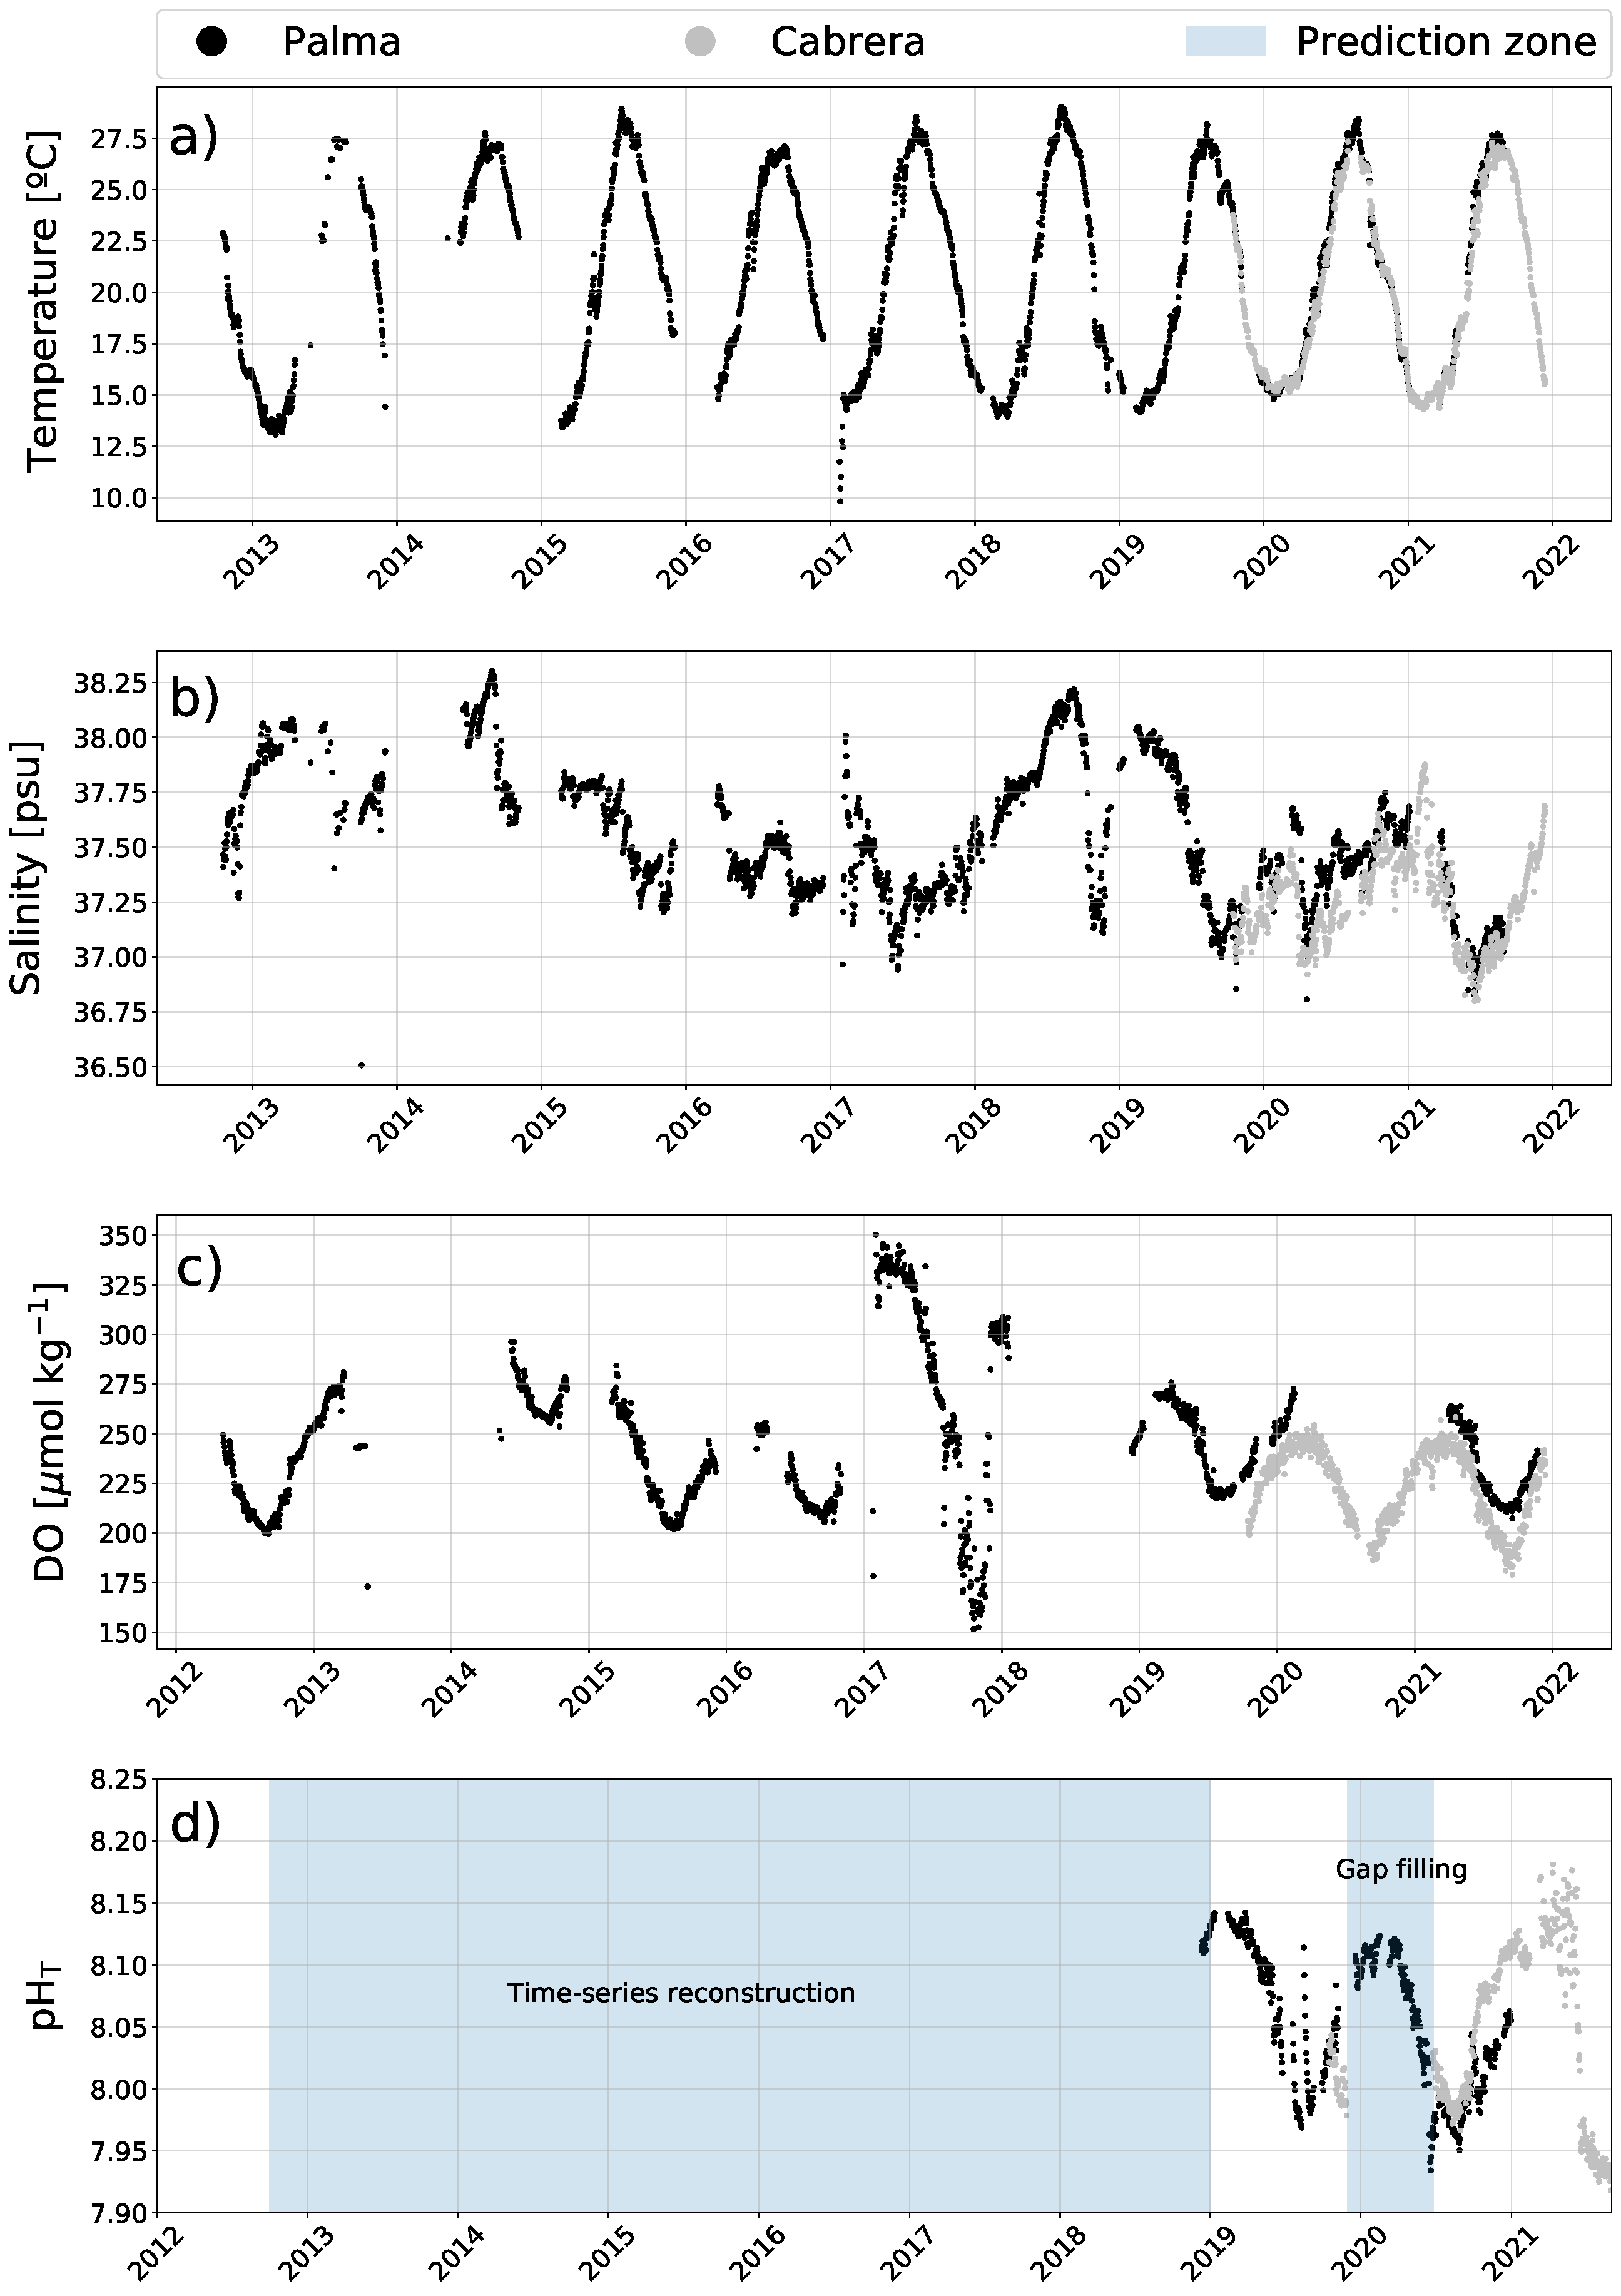
\includegraphics[width=0.7\textwidth]{Figures/Data_study.pdf}
    \caption{Daily averaged time series data from the Bay of Palma (black dots)
        and Cabrera stations (grey dots): a) Temperature (Cº), b) Salinity
        (psu), c)
        Dissolved oxygen (DO) values (${\mu\textrm{mol
                        kg}\textsuperscript{-1}}$) and
        d) pH\textsubscript{T} in pH units. The pH time series of the Bay of
        Palma will
        be reconstructed in the period 2012-2021 while only gaps will be filled
        in
        Cabrera, as marked in blue in the figure.}
    \label{fig:data}
\end{figure}

In both stations, temperature ranged from a minimum of 12.99 ºC to maximum
values of 29.07ºC from 2012 to 2021, with no observed differences between the
stations in Cabrera and the Bay of Palma (\cref{fig:data}(a)). The surface
water temperatures are a clear representation of the typical Mediterranean
climate seasonality with mild winters and warm to hot summers. Salinity did not
show a repetitive seasonal pattern between years in either stations. However,
in Cabrera salinity is slightly lower than in the Bay of Palma. During the data
acquisition period, the lowest salinity value of 36.83 was found in Cabrera and
highest of 38.30 in the Bay of Palma (\cref{fig:data}(b)).

The surface water of the coastal sites in the Balearic Sea in the Palma Bay
and the Cabrera stations was highly saturated with oxygen during all the
seasons, with DO concentrations up to  348.94 ${\mu \textrm{mol\,kg}^{-1}}$
during winter and of 169.66 ${\mu \textrm{mol\,kg}^{-1}}$ during the summer and
early autumn (\cref{fig:data}(c)). pH\textsubscript{T} values obtained starting
in December, 2018 to December, 2021 increased during winter reaching up to 8.18
pH units at \emph{in situ} temperature and decreasing to 7.91 pH units in
summer, with the highest variability and maximum and minimum values measured in
Cabrera (\cref{fig:data}(d)).

Considering sampling period of the additional (temperature and salinity)
and calculated parameters (Total Alkalinity; TA) was larger in the Bay of Palma
compared to Cabrera, we evaluate the linear tendencies with time for the Bay of
Palma variables. The sea surface temperature in the Bay of Palma increased with
a rate of 0.05 ± 0.03°C per year (R\textsuperscript{2}=0.0008,
\emph{p}-value=0.09) from 2012 to 2021, whereas the salinity decreased
significantly with -0.059 ± 0.002 psu per year (R\textsuperscript{2}=0.2456,
\emph{p}-value<0.001). The annual trend for TA, clearly related to the decrease
in surface salinity, showed a relevant decrease of -4.0 ± 0.4 ${\mu
            \textrm{mol\,kg}^{-1}}$ (R\textsuperscript{2}=0.0379,
\emph{p}-value<0.001),
supported by the discrete water samples for TA obtained during the period from
2019 to 2021  (\cref{fig:S1}).

\begin{figure}[H]
    \centering
    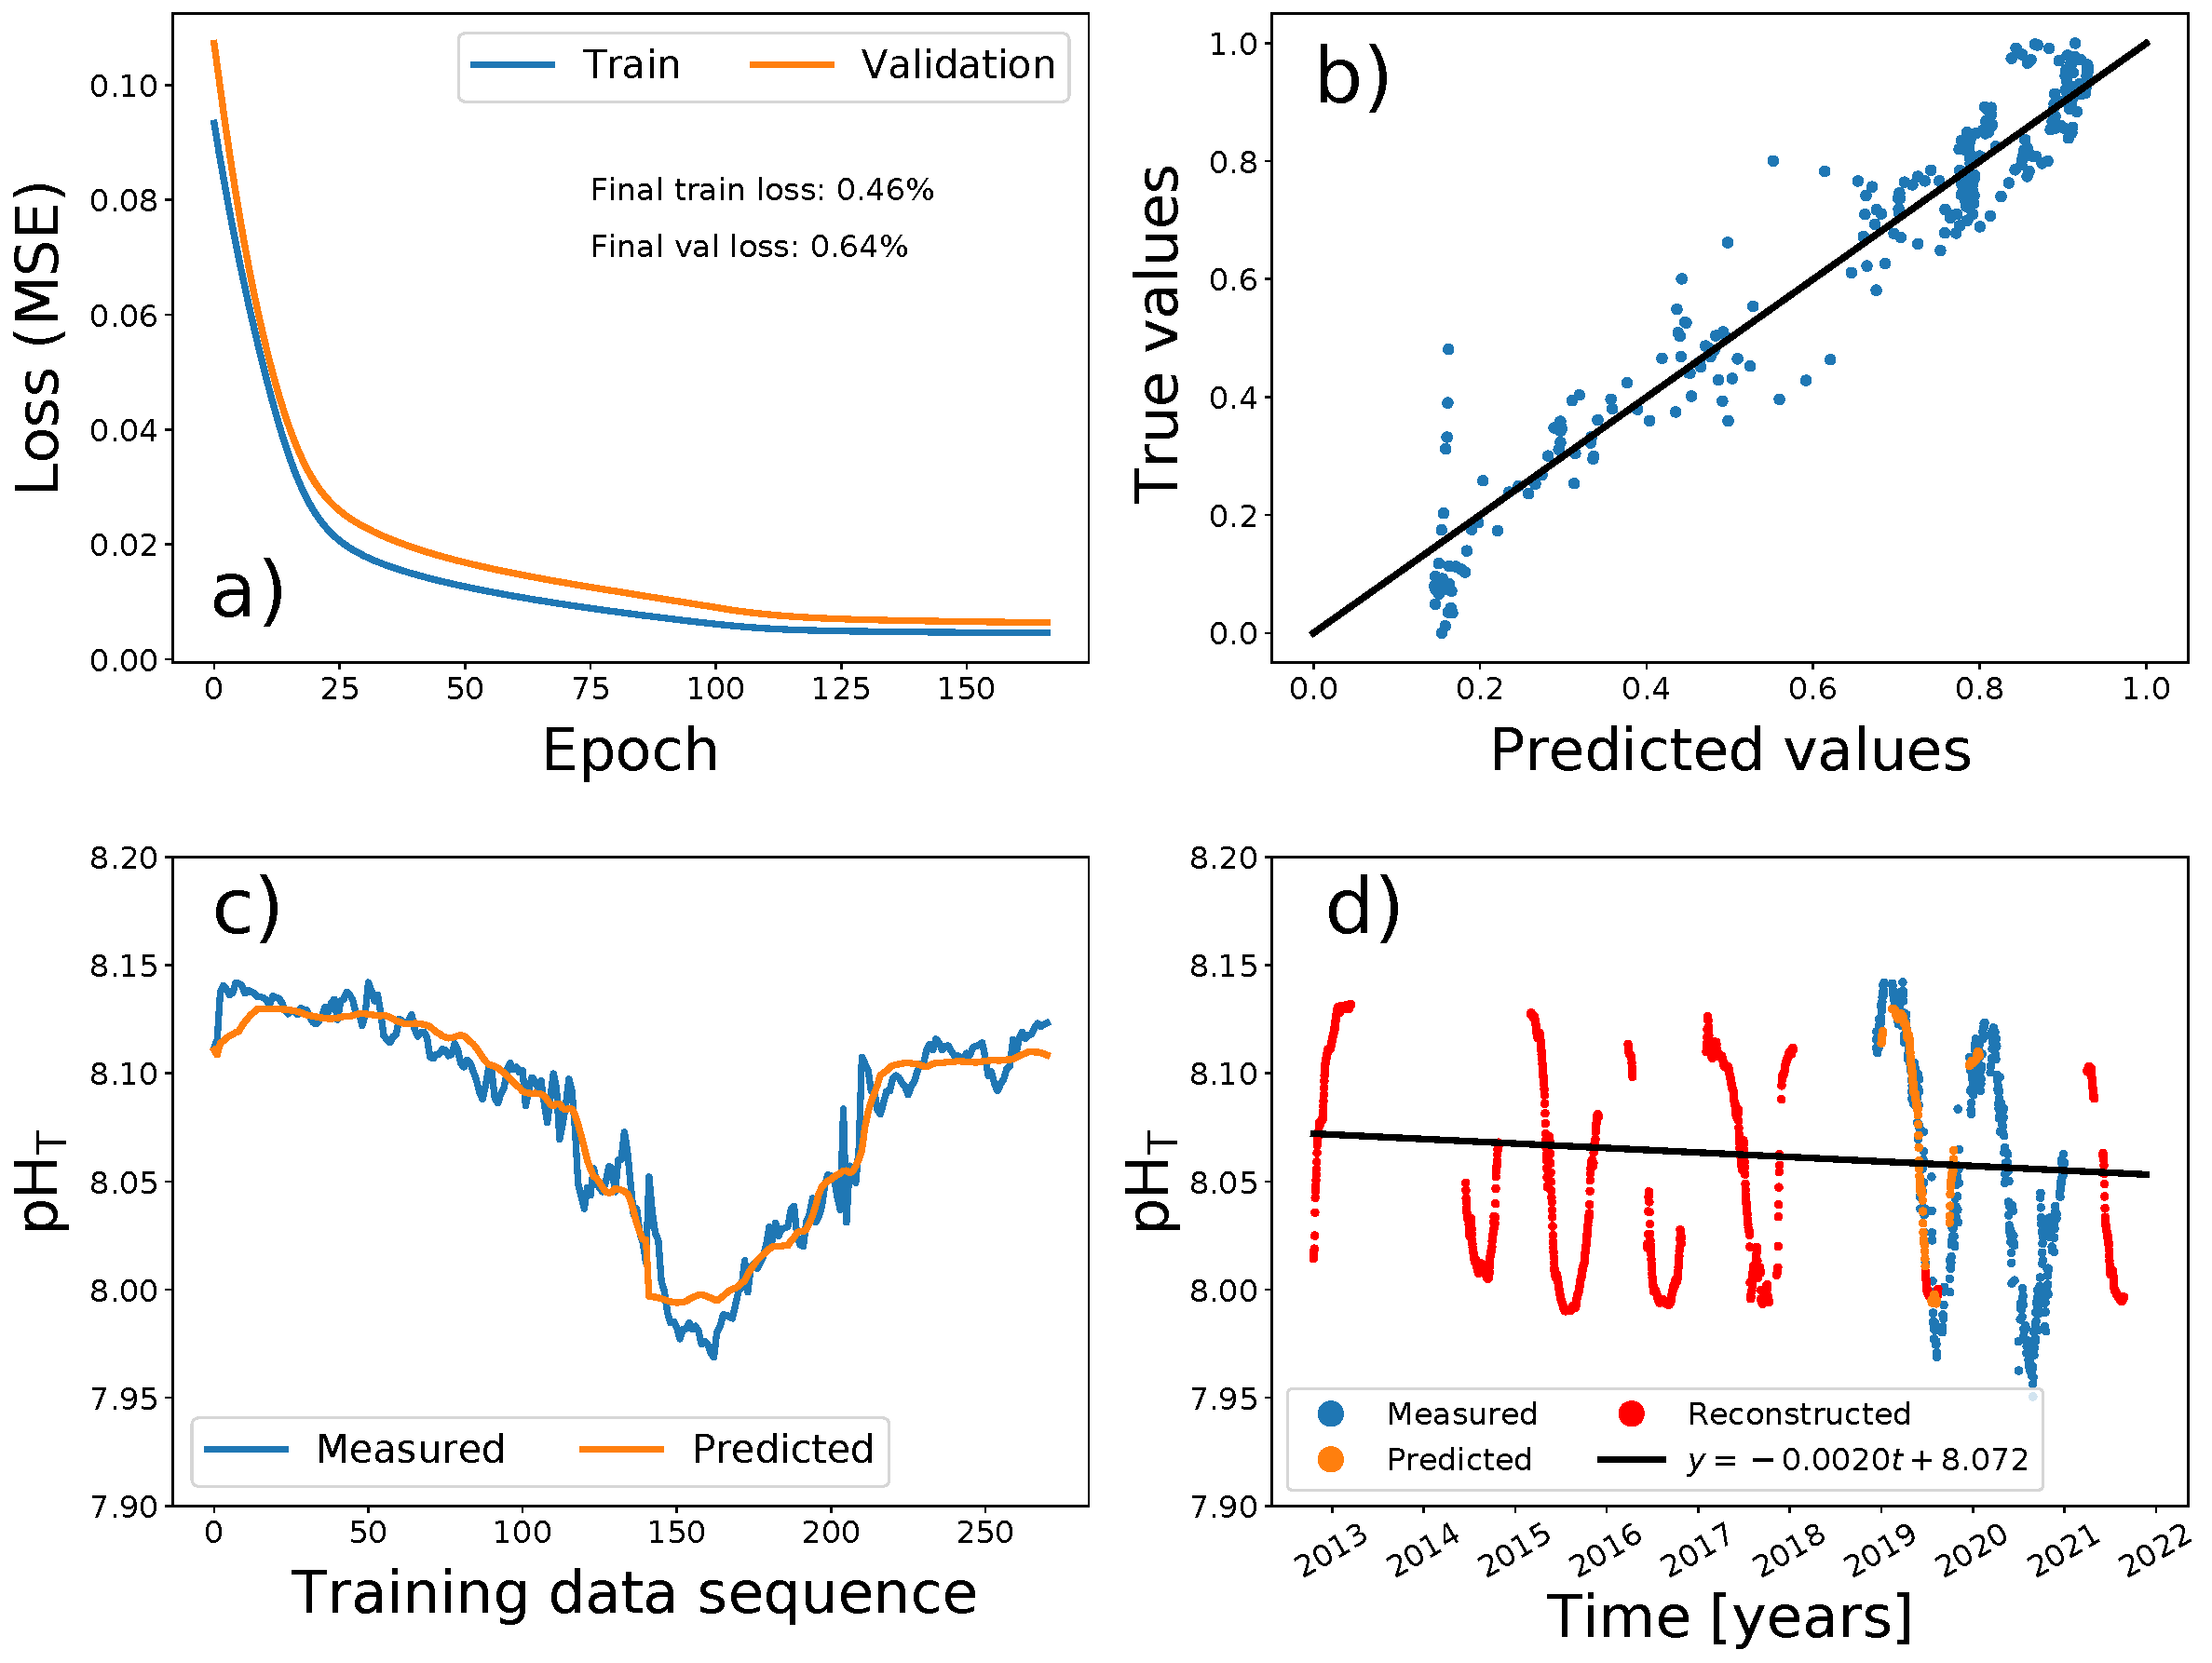
\includegraphics[width=0.85\textwidth]{Figures/Best_bidirectional_LSTM.pdf}
    \caption{Bidirectional LSTM neural network model applied to assess the
        decadal pH\textsubscript{T} trend in the Bay of Palma: a) Training
        process
        monitoring loss for both training and validation sets, b) Predicted
        pH\textsubscript{T} values against their true values where the black
        line is
        the reference for a perfect prediction, c) Predicted
        pH\textsubscript{T} time
        series in the training process (orange) and ground truth series (blue)
        and d)
        Final prediction for the decadal pH\textsubscript{T} time series using
        the
        output data of the trained model and the measured data. Measured pH
        data shown
        in blue, predicted data in the training process is shown in orange and
        reconstructed data is shown in red. The black line represents the
        decadal pH
        trend.}
    \label{fig:best_LSTM}
\end{figure}

\subsection{Reconstruction pH time series with Deep Learning}

The amount of available pH\textsubscript{T} data from both Palma Bay and
Cabrera stations is comparable and relatively short (mostly in Cabrera), but
the length of the additional ambient data (temperature, salinity and DO)
differs enormously between stations. Thus, there is a need to approach the time
series prediction problem for both sites with different objectives. Common to
both sites, a DL model with a RNN architecture will be developed to predict the
pH\textsubscript{T} time series from the accompanying ambient data
(temperature, salinity and dissolved oxygen), which are expected to be
correlated with pH\textsubscript{T} \cite{Fourrier2020,Broullon2021}. To avoid
the effect of site-specific correlations between ambient data and
pH\textsubscript{T} time series, the model will be trained independently with
the dataset of each location. In this way a proper model calibration is ensured
and the prediction power of the model is enhanced. In the Bay of Palma, the
model will be used to reconstruct the pH\textsubscript{T} time series from
2012, exclusively from the points for which the full set of ambient time series
data are available (\cref{fig:data}(d)). This is not possible in Cabrera, due
to the fact that no temperature, salinity and DO concentration is available
before 2019. Fortunately, these time series do not have the same gaps that the
pH\textsubscript{T} time series exhibits. Thus, we will use the model to fill
the gaps in the pH\textsubscript{T} time series from 2019 to present, as shown
in (\cref{fig:data}(d)).

\begin{figure}[H]
    \centering

    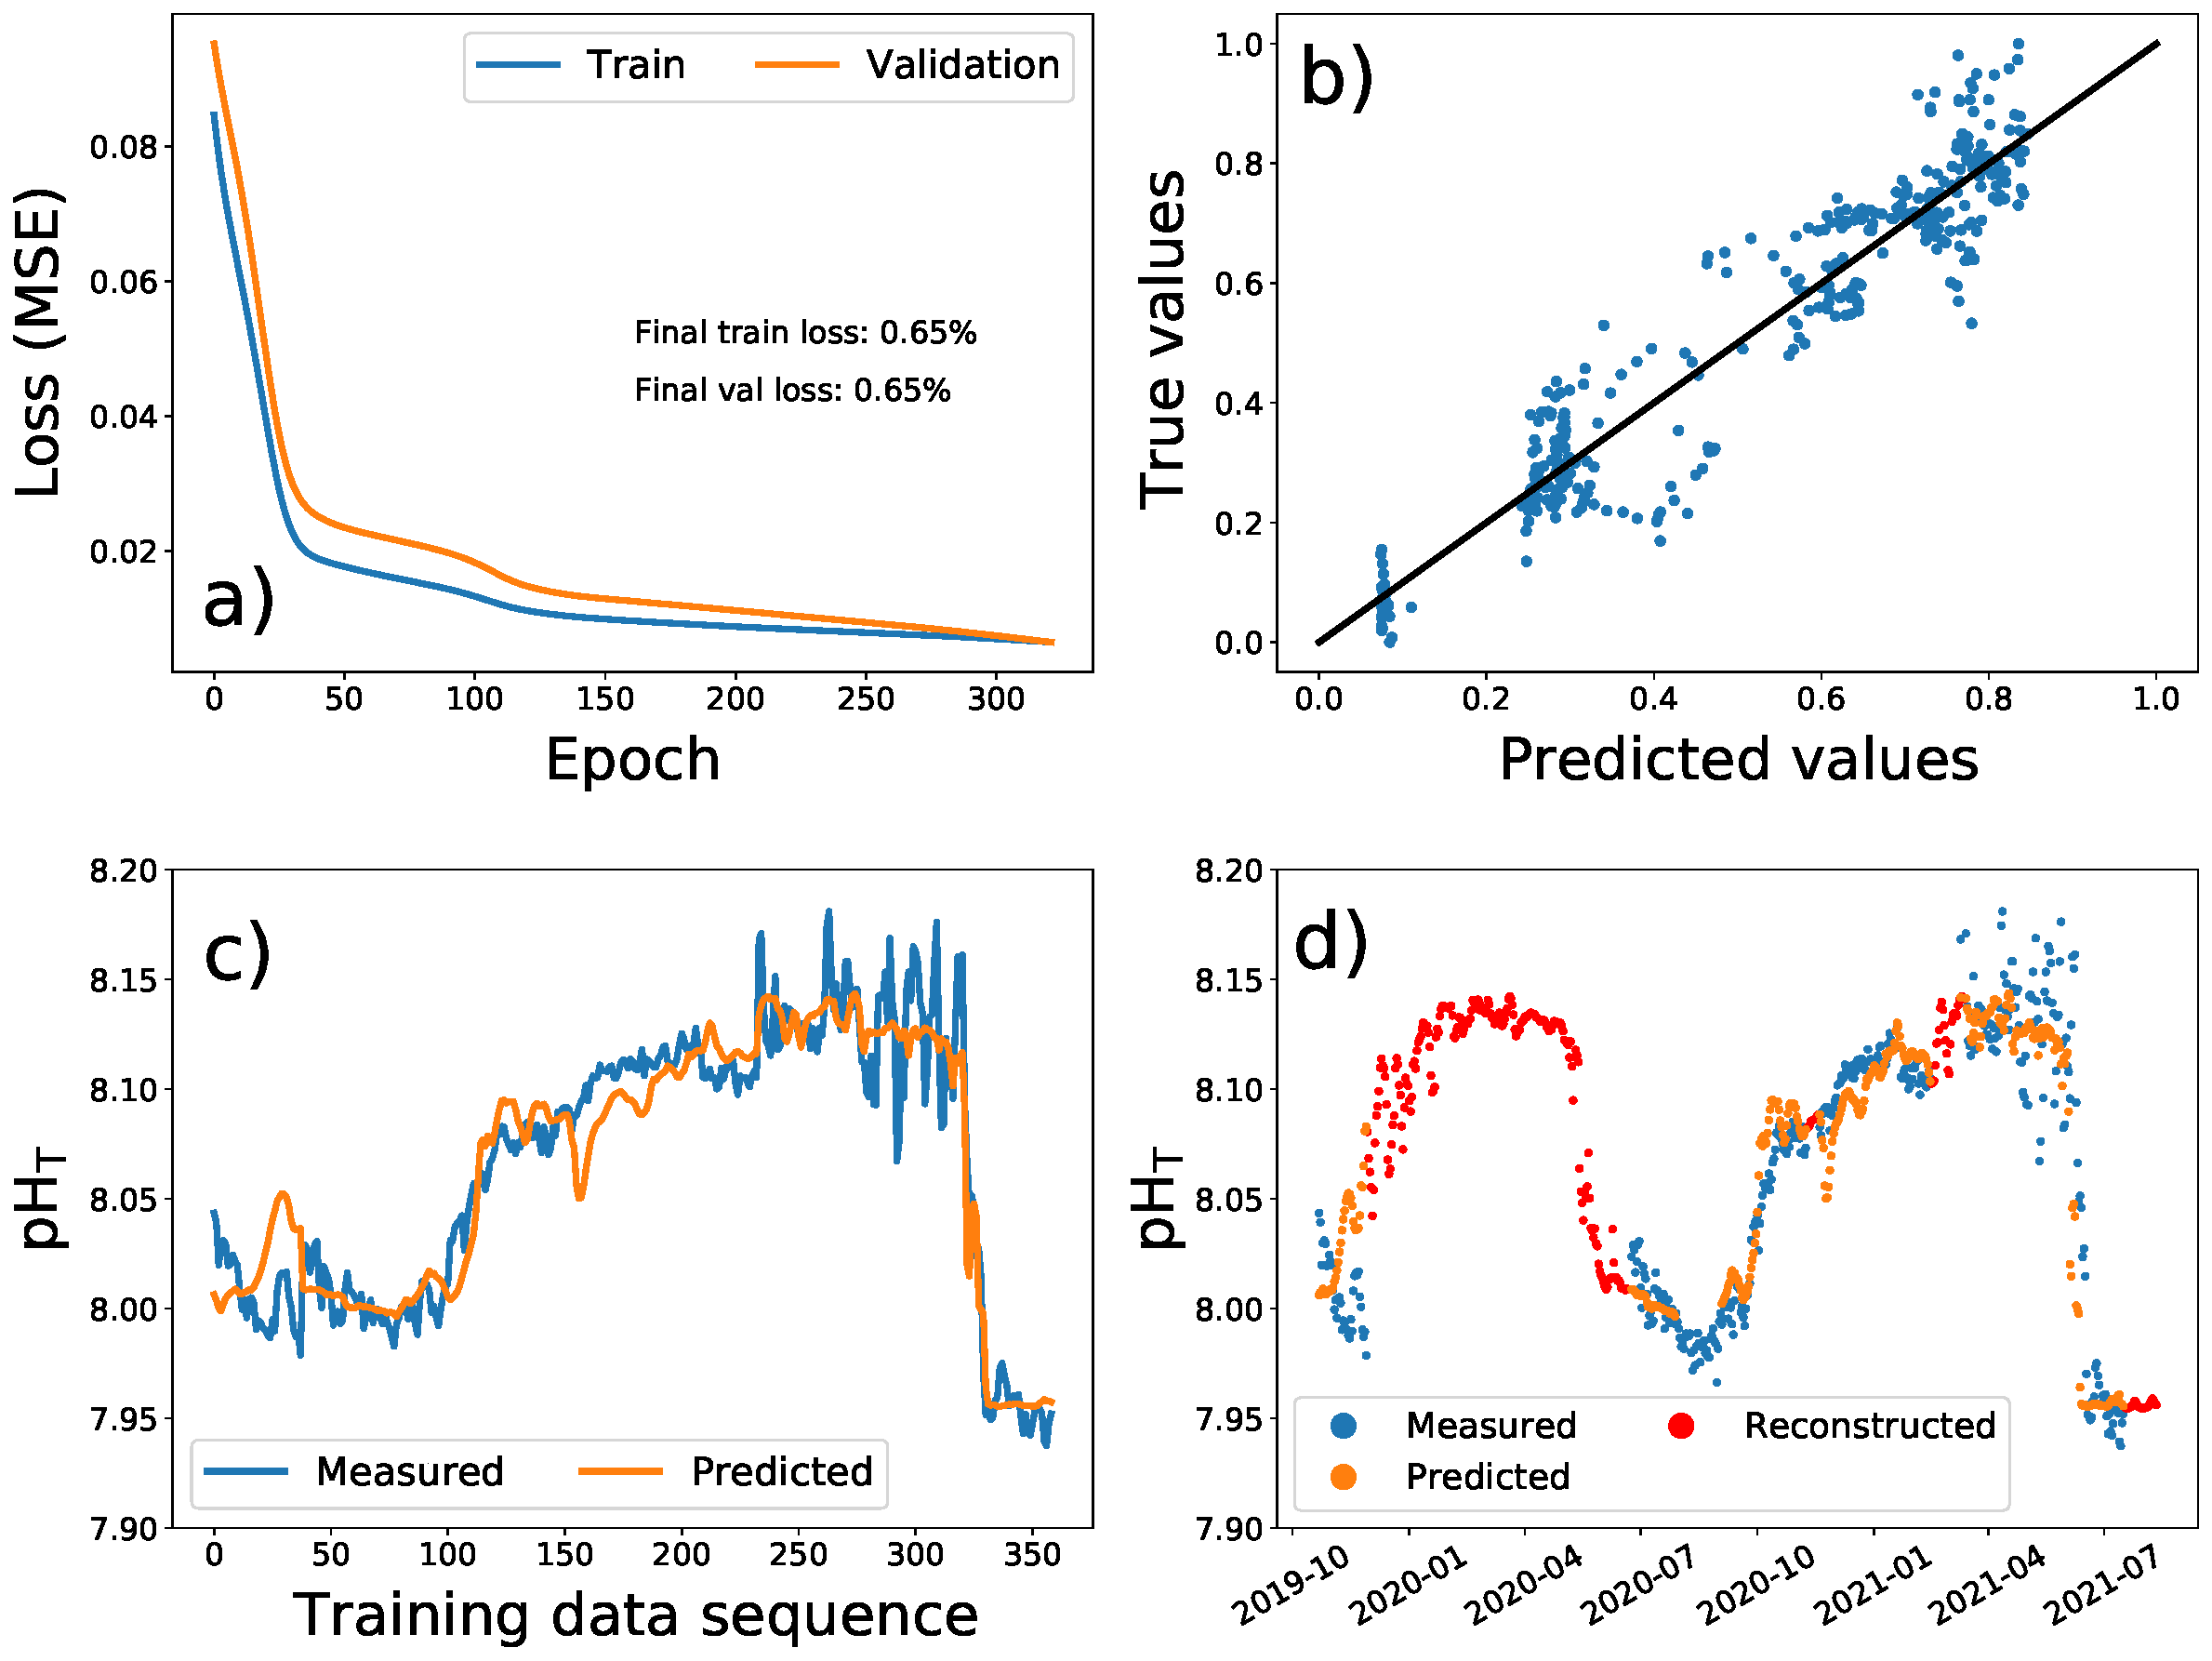
\includegraphics[width=0.85\textwidth]{Figures/bidirectional_LSTM_gap_filling.pdf}
    \caption{Bidirectional LSTM Neural Network model applied to fill the
        gaps in the pH\textsubscript{T} time series in Cabrera: a) Training
        process
        monitoring loss for both training and validation sets, b) Predicted
        pH\textsubscript{T} values against their true values where the black
        line is
        the reference for perfect prediction, c) Predicted pH\textsubscript{T}
        time
        series in the training process (orange) and ground truth series (blue)
        and d)
        Gaps in the pH\textsubscript{T} time series filled with the trained
        model
        (red), while measured pH\textsubscript{T} are shown in blue and
        predicted data
        in the training process shown in orange.}
    \label{fig:Cabrera_gap_filling}
\end{figure}

A BiDireccional Long Short-Term Memory (BD-LSTM) neural network
(\cref{fig:BD_LSTM_scheme}) was selected as the best recurrent neural network
architecture to reconstruct the pH\textsubscript{T} time series in the Bay of
Palma. The training process was successfully completed with no signs of
overfitting achieving less than 1\% error in both training and validation sets
(\cref{fig:best_LSTM}(a)). The BD-LSTM neural network was able to fairly
predict the majority of the individual pH data points in the time series,
although there are some deviations (\cref{fig:best_LSTM}(b)). Furthermore, the
time series pattern is perfectly captured by the neural network
(\cref{fig:best_LSTM}(c)). Notice the gaps in the reconstructed pH points (in
red) in (\cref{fig:best_LSTM}(d)), that are those for which the full ambient
time-series is not available. Finally, the reconstructed pH data using the
BD-LSTM model was used to assess the decadal trend of acidification in Palma
Bay, which yielded $-0.0020$ units of pH per year (black line in
(\cref{fig:best_LSTM}(d)). Indeed, to further characterize this decadal trend,
$1000$ independent training-prediction processes were carried out using a
BD-LSTM neural network. The results showed a mean slope of  $-0.0020 \pm
    0.00054$ for the decadal acidification trend (see methods).

Regarding the Cabrera data set, with the available ambient time series it
is only possible to fill the data gaps, task for which a BD-LSTM neural network
was also used. As for the Bay of Palma the training process was successfully
completed with no signs of overfitting, yielding less than 1\% error in both
training and validation dataset (\cref{fig:Cabrera_gap_filling}(a)). The model
fairly predicts most of the individual pH\textsubscript{T} data points in the
training dataset, showing some deviations as usual
(\cref{fig:Cabrera_gap_filling}(b)). The tendency of the time series is
perfectly captured by the model (\cref{fig:Cabrera_gap_filling}(c)) and thus
the gap can be filled with reliable data, red points in
(\cref{fig:Cabrera_gap_filling}(d)).

\section{Discussion}
The achievement of long time oceanographic data series suitable to evaluate
the effects of climate change constitutes a great operational effort which is
unequivocally accompanied by partial data loss due to multiple factors (human
and instrumental). The advances in the development of pH sensors are enabling
the acquisition of precise pH data without identified drift through highly
accurate indicator-based spectrophotometric methods \cite{seidel2008sensor}.
However, in order to determine OA trends, several years of quality seawater pH
data are needed, adding more difficulty to the vicissitudes inherent to field
work. Recently, the application of computational methods based on Deep Learning
(DL) is becoming a useful tool to fill the gaps due to data loss. Several
studies have implemented the DL methodology and successfully predicted
bio-optical and biogeochemical parameters
\cite{Bittig2018,Broullon2019,Broullon2021,Contractor2021,gregor2019comparative,lefevre2005comparison,Li2020nn,sauzede2017estimates,velo2013total}.
\\
Here, the application of a BiDireccional Long Short-Term Memory (BD-LSTM)
neural network to predict pH\textsubscript{T} from physical data, namely
temperature, salinity, and dissolved oxygen, the latter as a key indicator of
biological activity, permitted the reconstruction of gaps in the time series of
pH\textsubscript{T} and allowed the reconstruction of nine years of
pH\textsubscript{T} data. The BD-LSTM architecture has been proved extremely
effective in predicting sequence data, such as time series, as they combine the
information for both front and back directions of time
(Online Supplementary Information) \cite{graves2005}, and is more effective
(accurate
and stable) compared to unidirectional Long Short-Term Memory neural networks.
Therefore, in this study the BD-LSTM offered better estimation results over the
other neural networks considered to reconstruct time series but also in the
completion of missing data.\\
In the Cabrera station, the BD-LSTM applied permitted a reliable
reconstruction of the gaps in pH\textsubscript{T} data from December 2019 to
June 2020 (\cref{fig:data}(d)), constituting an advantageous methodology to
support the acquisition of long time series data without loosing accuracy, as
the model can reproduce pH\textsubscript{T} data with an error lower than 1\%
(\cref{fig:Cabrera_gap_filling}(b)), closely following the annual variability
of the observations (\cref{fig:Cabrera_gap_filling}(d)).\\
The ability of the BD-LSTM to reconstruct time series was observed through
the reconstruction of nine years of pH\textsubscript{T} data in the Bay of
Palma station (\cref{fig:best_LSTM}(d)). The modeled pH\textsubscript{T} data
combined with the observations allowed the accomplishment of a long pH time
series in order to estimate a pH trend, seasonally adjusted through a
sinusoidal fitting, with a rate of decrease of $0.0020\pm 0.00054$ pH units per
year ($R^2=0.1$, \emph{p}-value$<0.001$,
\cref{fig:seasonally_adjusted_fit_pH}), and represents the first estimate of pH
trend obtained in the Balearic coastal Sea. Additionally, we applied a linear
fit on the reconstructed pH time series obtaining trend of $-0.0025\pm 0.00053$
y\textsuperscript{-1}($R^2=0.01$, \emph{p}-value$<0.001$). This fit was
discarded, because it was shown to introduce a bias in the pH decrease trend.
\\
The observed pH decrease in the Balearic Sea coastal area is well aligned
with OA trends reported for open ocean areas, from –0.0013 pH units
yr\textsuperscript{-1} in the Munida station (New Zealand) to the high trend
found in the Cariaco Basin station up to –0.0026 pH units per
year\cite{Bates2014}. The processes associated with the increased pH decline in
the Cariaco Basin where related to the upwelling of Subtropical Underwater,
rich in dissolved inorganic carbon, thus lowering the pH.\\
In the Mediterranean Sea, previous annual estimates in open ocean areas
ranged from -0.003 to -0.0044 \cite{yao2016,Flecha2015}, reflecting the effect
of the hydrodynamical and biogeochemical characteristics of the basin on the
seawater pH variability\cite{lee2011,Palmieri2015,schneider2010}. However, it
can be assumed that differences in physical oceanography and ecological
processes between areas may modulate local changes of pH. In a coastal
Mediterranean area located in the northwestern basin, close to
Villefranche-sur-Mer, a rate of pH change of $-0.0028\pm 0.0003$ pH units
yr\textsuperscript{-1} was observed\cite{Kapsenberg2017} and attributed
principally to atmospheric forcing and secondly to increased warming.
The calculated trend of pH decrease due to the atmospheric
CO\textsubscript{2} growth during the period of this study, from 2013 to 2021,
was of $0.0025\pm 0.0002$ pH units per year (R\textsuperscript{2}=0.95,
\emph{p}-value<0.001), consistently related to the seawater pH decline.
Therefore these analyses suggest that the atmospheric forcing is the main
driver responsible for the pH decreasing trend trend found in the surface
coastal Balearic Sea. Subsequently, the difference between the seawater pH
decreasing trend obtained and the pH trend calculated from the atmospheric
levels could be related to natural biogeochemical processes, not distinctly
quantifiable with the available length of the Bay of Palma pH time series.\\
In addition, the effect of temperature on surface ocean pH, occurring
directly through the temperature dependence of the seawater CO\textsubscript{2}
chemistry, as changes in temperature and salinity influence the equilibrium
constants of the oceanic CO\textsubscript{2} system and indirectly through
air-sea exchange of CO\textsubscript{2}, can be considered. The influences of
these two temperature processes on surface ocean pH has been found responsible
of a 50\% of the increase in [H\textsuperscript{+}] ions, thus a pH decrease,
in the surface layers of the Iceland and Irminger
Seas\cite{perez2021contrasting}. In the Mediterranean Sea northwestern basin, a
temperature increase of $0.072\pm 0.022$ °C yr\textsuperscript{-1} was
estimated to be responsible for a 40 percent of the pH
decrease\cite{Kapsenberg2017}. The obtained temperature variability in the
Balearic Sea coastal area during this study was of $0.035\pm 0.008$
($R^2=0.008$, p-value $<0.001$, \cref{fig:seasonally_adjusted_fit_T}),
indicating that temperature-driven changes could also be assumed to affect the
pH trend.\\
The observed seasonal variability of the data, presented a
pH\textsubscript{T} increase from 7.91 during summer up to 8.18 pH units
(\cref{fig:data}(d)) in winter seasons, clearly followed by the TA values
(\cref{fig:S1}). Seasonal changes in TA levels in the study area are ranging
from around 2350 to 2550 ${\mu \textrm{mol\,kg}^{-1}}$ (\cref{fig:S1}), largely
overtaking the seasonal differences reported previously in the Balearic Sea of
up to 50 ${\mu \textrm{mol\,kg}^{-1}}$ in
total\cite{cossarini2015spatiotemporal}. This discrepancy in variability could
be explained by the intense metabolic processes at the coastal location of the
Bay of Palma station. This shallow area has a strong coverage of
\emph{Posidonia oceanica}, which due to its high ecosystem
production\cite{koopmans2020high} could be triggering an increase of pH and TA
levels, as seen in salinity normalized TA values (NTA, not shown) during
winter-spring, due to the uptake of nitrate and phosphate and the calcium
carbonate dissolution\cite{barron2006organic,cossarini2015spatiotemporal}, and
during summer, related to the lower community
production\cite{champenois2012seasonal} an NTA-pH
decrease\cite{cossarini2015spatiotemporal}. \\
Another result from this study worth to mentioning is the obtained
decreasing TA trend in the Bay of Palma of -4.0±0.4 ${\mu
            \textrm{mol\,kg}^{-1}}$ per year. Although the Western
Mediterranean is
characterized with lower total alkalinity values in relation to the rest of the
basin, resulted from the nearby influence of Atlantic waters, less salty with
low-alkalinity water\cite{RIVARO2010236,hassoun2015modeling}, was not expected
to influence decreasing decadal TA values. In the northwestern basin, TA values
increased over time at a rate of 2.08±0.19 ${\mu \textrm{mol\,kg}^{-1}}$
yr\textsuperscript{-1}. In the Balearic Sea, the decreasing TA confirm the
Atlantic forcing on the alkalinity values and the negligible TA discharges due
to rivers in the Balearic Islands. There is a marked south-to-north surface
gradient in the western region coupled with the west-to-east gradient of
alkalinity in the Mediterranean Sea related to the Atlantic
influence\cite{cossarini2015spatiotemporal,Gemayel2015}. Due to a well
established linear relationship of TA and
salinity\cite{schneider2007alkalinity} and the calculated origin of our
values\cite{Gemayel2015} we cannot neglect the strong TA related to the
salinity decrease in the study area of -0.059±0.002 psu per year
(R\textsuperscript{2}=0.25, \emph{p}-value<0.001). This rate is in agreement
with the salinity decrease found at the coastal site at Villefranche-sur-Mer
(-0.0017±0.0044 psu yr\textsuperscript{-1}).\cite{Kapsenberg2017}.
Notwithstanding, the intense salinity decrease observed in the Bay of Palma can
be linked to a decrease of the intensity of the southern spreading of the
Balearic Current trough the Ibiza channel (located between Ibiza and Mallorca
Islands) driven by mesoscale processes, and the prevalence of new Atlantic
Water coming from the Strait of Gibraltar\cite{millot1999circulation}.
Although, this observation is out of the scope of this study and therefore
further investigation is needed.\\
In summary, this work pointed out the useful use of DL techniques,
specifically the BD-LSTM architecture, to reconstruct pH data relevant to
evaluate seasonal pH variability and to elucidate the climate change
consequences, as the OA effect, in a coastal area of the Balearic Sea, which
can be extended to the coastal areas of the Western Mediterranean Sea Basin.
Nevertheless, future research is necessary to assess and confirm these regional
trends, which highlights the importance of maintaining the time series
monitoring networks whose data are the base of this study.

\section{Methods}
\subsection*{Study area}
We monitored two coastal stations located in the Archipelago of the
Balearic Islands in the Western Mediterranean Sea (\cref{fig:1}). One site was
positioned within the Bay of Palma (39º29.57088’N; 2 º42.02430’E
\cref{fig:1}(b)) at a fixed station consisting of an oceanographic buoy managed
by the Balearic Islands Coastal Ocean Observing and Forecasting System (SOCIB;
https://www.socib.eu/). Here meteorological, hydrological and hydrodynamic data
are collected with an hourly frequency since October 2012. The buoy is located
at the surface over 20m bottom depth. The Bay of Palma is a large bay with a
surface area of 217 km\textsuperscript{2} and approximately 30\% seagrass
cover\cite{gazeau2005whole}. The second station was located at 4m depth on a
mooring line over 8m bottom depth deployed in the Marine and Terrestrial
National Park of the Archipelago of Cabrera (39º 9.08217’N; 2º 57.04767’E;
\cref{fig:1}(b)). The mooring line is in a small bay of just under 1
km\textsuperscript{2} and full protection with the largest meadow of the
archipelago, covering 89.1\% of the surface area between 0-10m
depth\cite{marba2002effectiveness}. Neither site has important freshwater
inputs. Both stations are part of the Balearic Ocean Acidification Time Series
(BOATS) network included in the Interdisciplinary Thematic Platform: Water:iOS
(https://pti-waterios.csic.es/).

\begin{figure}[H]
    \centering
    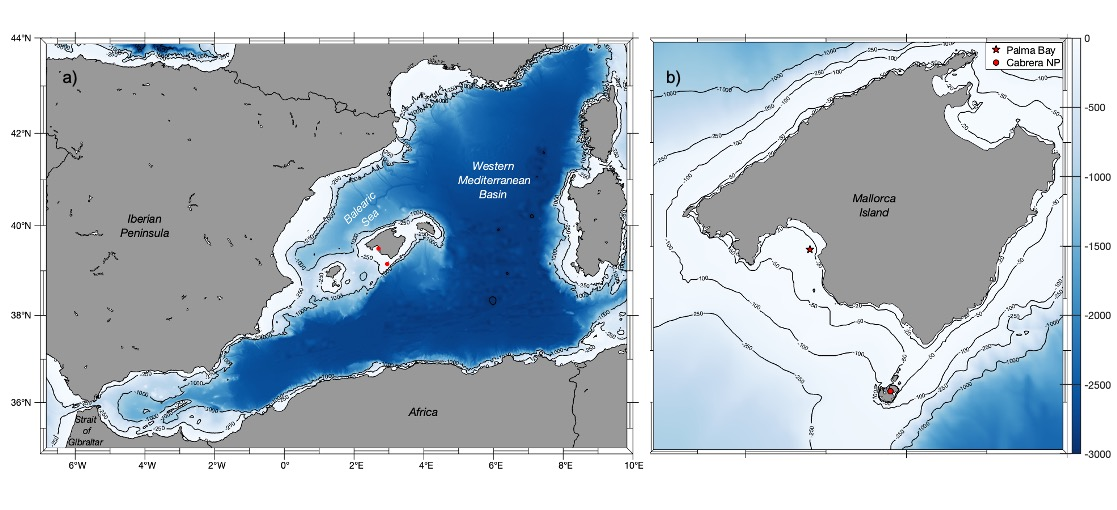
\includegraphics[width=\textwidth]{Figures/Fig_1.jpg}
    \caption{a) Map of the stations location in the Western Mediterranean Sea
        Basin (red dots) and b) detailed location of the Bay of Palma (red
        star) and
        the Cabrera National Park (Cabrera NP, red dot) study sites. Maps were
        developed with the MATLAB\textsuperscript{\textregistered} R2010b
        software
        (https://mathworks.com) by using the M\_Map
        toolbox\cite{pawlowicz2020m_map}.}
    \label{fig:1}
\end{figure}

\subsection{Data collection}
In both stations a SAMI-pH (Sunburst Sensors LCC) was attached, at 1 m in
the Bay of Palma and at 4 m depth in Cabrera. The pH sensors were measuring pH,
in the total scale (pH\textsubscript{T}), hourly since December 2018 in the Bay
of Palma and since November 2019 in Cabrera. The sensor precision and accuracy
are <0.001 pH and ± 0.003 pH units, respectively. Monthly maintenance of the
sensors was performed including data download and surface cleaning.\\
Temperature and salinity from the Bay of Palma oceanographic buoy was
obtained from October 2012 and for the Cabrera mooring line from November 2019
with a CT SBE37 (Sea-Bird Scientific©) in both stations. Accuracy of the CT is
± 0.002°C for temperature and ± 0.003mS cm\textsuperscript{-1} for
conductivity.  Additionally, oxygen data from a SBE 63 (Sea-Bird Scientific ©)
sensor attached to the CT in Cabrera and from a YSI 6600V2-4 Multiparameter
Water Quality Sonde with a 6450 ROX DO sensor (Yellow Spring Instruments Inc.
©)\cite{tintore2022} and a miniDot (PME, Inc. ©) in the Bay of Palma were used.
Accuracy of oxygen sensors is ± 2\%, ± 1\% and ± 5\% for the SBE 63, the YSI
and the miniDot, respectively.\\
Periodically water samplings for dissolved oxygen (DO), pH in total scale
at 25°C (pH\textsubscript{T25}) and total alkalinity (TA) were obtained during
the sensor maintenance campaigns. DO and (pH\textsubscript{T25}) samples were
collected in order to validate the data obtained by the sensors.\\
DO concentrations were evaluated with the Winkler method modified by Benson
and Krause (1983) \cite{Benson_Krause_1984} by potentiometric titration with a
Metrohm 808 Titrando with an accuracy of the method of ± 2.9 ${\mu
            \textrm{mol\,kg}^{-1}}$ and with an obtained standard deviation
from the
sensors data and the water samples collected of ± 5.9 ${\mu
            \textrm{mol\,kg}^{-1}}$.\\
pH\textsubscript{T25} data was obtained by the spectrophotometric method
with a Shimadzu UV-2501 spectrophotometer containing a 25°C-thermostated cells
with unpurified \emph{m}-cresol purple as indicator following the methodology
established by Clayton and Byrne (1993)\cite{Clayton_Byrne_1993} by using
Certified Reference  Material (CRM Batch \#176 supplied by Prof.  Andrew
Dickson, Scripps  Institution  of  Oceanography, La  Jolla,  CA,  USA). The
accuracy obtained from the CRM Batch was of ±0.0051 pH units and the precision
of the method  of ±0.0034 pH units. The mean difference between the SAMI-pH and
discrete samples was of 0.0017 pH units.\\
TA samples were collected in $\SI{50}{ml}$ Falcom vials and poisoned with
$\SI{20}{\mu L}$ of HgCl\textsubscript{2} and determined by open cell
potentiometric titration with a Titrando 808 (Metrohm) following the Standard
Operation Procedure (SOP) 3b\cite{Dickson2007}.
TA values were also calculated from the temperature and salinity values
obtained in the Bay of Palma from 2012 by using a second-order polynomial model
for TA specifically described for the Mediterranean Basin \cite{Gemayel2015}.
\\
pH values due to the atmospheric CO\textsubscript{2} levels were estimated
by using the CO2SYSv3 program\cite{Sharp2020}, with the most internally
consistent and preferred carbon \cite{mehrbach1973,dickson1987} and sulfate
dissociation constants\cite{dickson1990} for current surface ocean
studies\cite{woosley2021}, with the Bay of Palma \emph{in situ} temperature and
salinity, the calculated TA values and the atmospheric CO\textsubscript{2}
levels converted from dry air to wet\cite{weiss1980nitrous} as inputs. Carbon
dioxide (CO\textsubscript{2}) atmospheric molar fraction used was obtained from
the monitoring station of Lampedusa (LMP), Italy of the NOAA (National Oceanic
and Atmospheric Administration, USA) monitoring network\cite{Duglokencky2021}.

\subsection{Data processing}

Once data was validated, several processing steps were performed to ensure
an optimal training process for the neural network models. First, all the data
of the time series were re-sampled by averaging the data points obtaining a
daily frequency. Afterwards, a standard feature-scaling procedure (min-max
normalization) was applied to every feature (Temperature, Salinity and Oxygen)
and to pH\textsubscript{T}. Finally, we built our training and validations sets
as tensors with dimensions $(\textrm{batch}_\textrm{size},
    \textrm{window}_\textrm{size}, N_{\textrm{features}})$,  where
$\textrm{batch}_\textrm{size}$ is the number of examples to train per
iteration, $\textrm{batch}_\textrm{size}$ is the number of past and future
points considered and $N_{\textrm{features}}$ is the number of features used to
predict the target series. Temperature values below $T=12.5$ \textdegree C were
discarded as they are considered outliers in sensor data outside the normal
range in the study area.

\subsection{Computing the trend of seasonal data}

The trend of seasonal time-series is often computed by means of statistical
methods based on moving averages or more advanced techniques such as the
Seasonal Trend Decomposition Loess \cite{cleveland1990stl}. Nevertheless, these
procedures do not work with gappy time series, so that a different approach is
needed. In this work we fitted the following oscillatory function with trend to
our data:
\begin{equation}\label{eq:seasonal_fit}
    y(t)=A\sin(\omega t+\phi)+Bt+C \ ,
\end{equation}
where the parameter $B$ corresponds to the trend of the data.\\
Moreover, after this fit, the seasonal component ($A\sin(\omega t + \phi)$)
can be removed from the original time-series and a standard linear regression
can be performed to the transformed data to obtain the trend (which is exactly
$B$) with the $R^2$ and \emph{p}-value estimates given by the linear regression
(\cref{fig:seasonally_adjusted_fit_pH,fig:seasonally_adjusted_fit_T}).

\subsection{Selecting the best neural network architecture}

Several recurrent neural network (RNN) architectures were considered as
candidates to reconstruct the pH time series, including a Simple Recurrent
neural network (SRNN), Long-Short Term Memory (LSTM), BiDirectional LSTM
(BD-LSTM, (\cref{fig:BD_LSTM_scheme}) and BiDirectional Gated Recurrent Unit
(BD-GRU).\\
Initially, manual tests were performed on each architecture to determine
the optimal set of parameters that yielded the best possible results. These
tests were based on minimizing the errors in both training and validation set
while avoiding overfitting. To avoid overfitting we implemented automated
callbacks to stop the training process whenever the validation loss increased
or crossed the training loss. During this test we determined the minimum number
of nodes, which helps in avoiding overfitting and the minimum window size,
which allows to use the most possible number of data points for training and
prediction. All the RNNs were trained in batches of size 32. To enhance clarity
and accessibility, the optimal values obtained for the more relevant parameters
are summarized in \cref{tab:NNs_parameters}.
\begin{table}[H]
    \centering
    \caption{Optimal parameters used for the different RNN architectures}
    \label{tab:NNs_parameters}
    \resizebox{\textwidth}{!}{%
        \begin{tabular}{l|cccccccc} \hline \hline
                                         & \textbf{Hidden layers} &
            \textbf{Nodes/Cells}         & \textbf{Window size}   &
            \textbf{Activation function} &
            \textbf{Output function}     &
            \textbf{Loss}                & \textbf{Learning rate} &
            \textbf{Optimizer}
            \\ \hline
            \textbf{SRNN}                & 1                      & 3   & 6
                                         &
            Tanh                         & Sigmoid                & MSE & 0.01
                                         & Adam
            \\
            \textbf{LSTM}                & 1                      & 3   & 6
                                         &
            Tanh                         & Sigmoid                & MSE & 0.01
                                         & Adam
            \\
            \textbf{BD-LSTM}             & 1                      & 3   & 6
                                         &
            Tanh                         & Sigmoid                & MSE & 0.01
                                         & Adam
            \\
            \textbf{BD-GRU}              & 1                      & 1   & 6
                                         &
            Tanh                         & Sigmoid                & MSE & 0.01
                                         & Adam
            \\
            \hline \hline
        \end{tabular}%
    }
\end{table}
\noindent In order to identify the best-performing architecture an
automated procedure was developed to statistically compare the outputs of each
model. Each architecture was trained in $1000$ independent processes, ensuring
a final training mean-squared error of less than $0.8\%$ while avoiding
overfitting implementing the previously mentioned callbacks. The code used for
the analysis can be found in \cite{CODE}.\\
In \cref{tab:architecture_comparison} a summary of the statistical results
obtained for each architecture is presented. All architectures provide similar
training and validation errors and provide similar results for the decadal
pH\textsubscript{T} trend, predicting a slope of around $-0.0030$ pH units per
year with an intercept of $8.07$ pH units. However, the BD-LSTM turns out to be
the architecture providing most accurate (smallest training and validation
errors) and precise (smallest statistical error) results
(\cref{fig:BD_LSTM_scheme}). Thus, we selected the BD-LSTM neural network as
the best architecture to reconstruct the pH\textsubscript{T} time series.
Data corresponding to the Bay of Palma were used in the selection of the
best neural network architecture.

\begin{table}[H]
    \centering
    \caption{Statistical comparison between different RNN architectures}
    \label{tab:architecture_comparison}
    \resizebox{\textwidth}{!}{%
        \begin{tabular}{l|cccccc} \hline \hline
                                      & \textbf{Slope}           &
            \textbf{Intercept}        & \textbf{Training error}  &
            \textbf{Validation error} & \textbf{Training epochs} &
            \textbf{Training time}
            \\ \hline
            \textbf{RNN}              & -0.0021 $\pm$ 0.00077    & 8.07 $\pm$
            0.006                     & 0.54
            $\pm$ 0.08                & 0.72 $\pm$ 0.12          & 293 $\pm$ 95
                                      & 15.52 $\pm$ 4.75
            \\
            \textbf{LSTM}             & -0.0018 $\pm$ 0.00067    & 8.06 $\pm$
            0.005                     & 0.49
            $\pm$ 0.03                & 0.68 $\pm$ 0.05          & 245 $\pm$ 68
                                      & 17.55 $\pm$ 4.21
            \\
            \textbf{BD-LSTM}          & -0.0020 $\pm$ 0.00054    & 8.07 $\pm$
            0.004                     & 0.46
            $\pm$ 0.03                & 0.64 $\pm$ 0.04          & 167 $\pm$ 45
                                      & 15.13 $\pm$ 3.00
            \\
            \textbf{BD-GRU}           & -0.0020 $\pm$ 0.00066    & 8.07 $\pm$
            0.005                     & 0.51
            $\pm$ 0.07                & 0.74 $\pm$ 0.10          & 347 $\pm$ 95
                                      & 27.68 $\pm$ 6.84
            \\ \hline \hline
        \end{tabular}%
    }
\end{table}

\noindent The code and data used to determine the best neural network
architecture can be found in a GitHub repository \cite{CODE_ph}.
